\paragraph{random\_access}

RandomAccessGate is used for verify that an element matches a value in the list.

\begin{figure}[!ht]
    \centering
    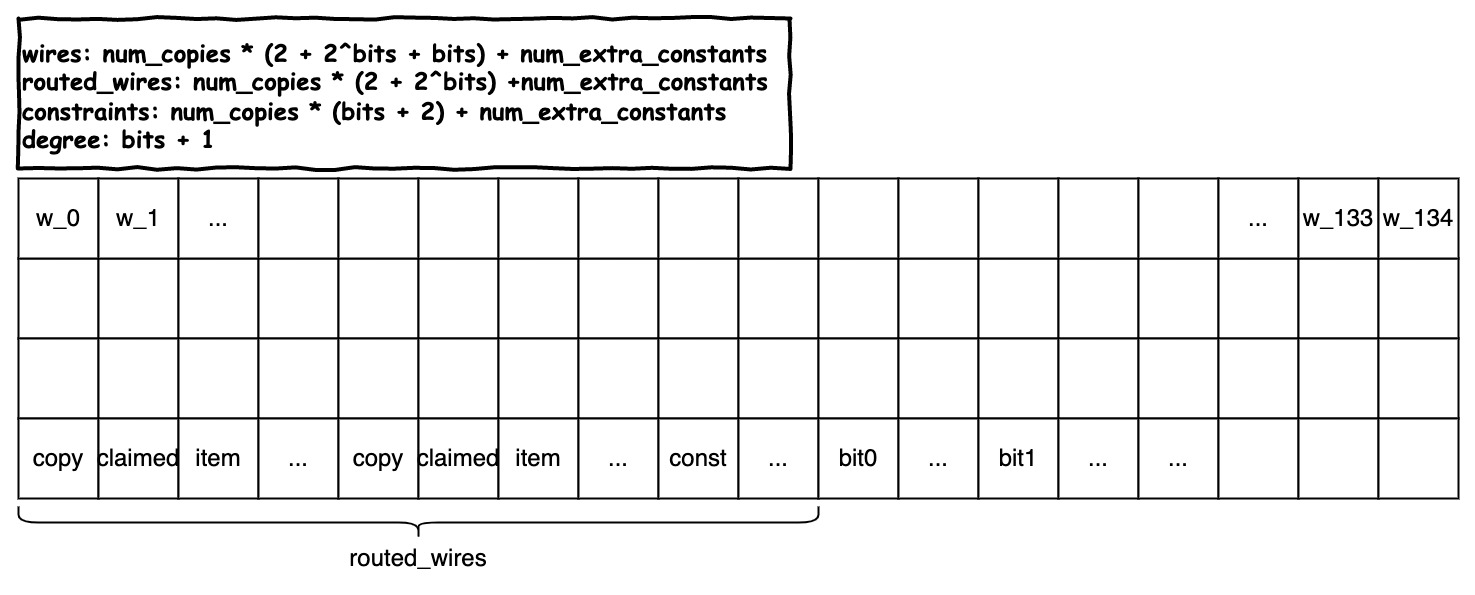
\includegraphics[width=0.6\textwidth]{gates/random_access.jpeg}
    \caption{RandomAccessGate}
    \label{fig:random-access}
\end{figure}

\begin{itemize}
    \item item: list items.
    \item copy: index of target element in the list
    \item claimed: target element
    \item bit\_i: bits for the i-th copy
\end{itemize}

For each copy:
\begin{itemize}
    \item Constrain bits are 0 or 1. -- bits constraints for each copy, A total of num\_copied*bits constraints.
    \begin{lstlisting}[language=rust]
for &b in &bits {
    constraints.push(builder.mul_sub_extension(b, b, b));
}
    \end{lstlisting}
    \item Constraint copy consists of bits. -- 1 constraint for each copy, A total of num\_copied constraints.
    \begin{lstlisting}[language=rust]
let reconstructed_index = bits
    .iter()
    .rev()
    .fold(zero, |acc, &b| builder.mul_add_extension(acc, two, b));
constraints.push(builder.sub_extension(reconstructed_index, access_index));
    \end{lstlisting}
    \item For each bits, reconstruct items with 2-elements-tuple, select first element when bit is 0 and select second when bit is 1.
    After the bits round, only one element remains, that is, the index element corresponding to bits, constraint it with claimed.
    \begin{figure}[!ht]
        \centering
        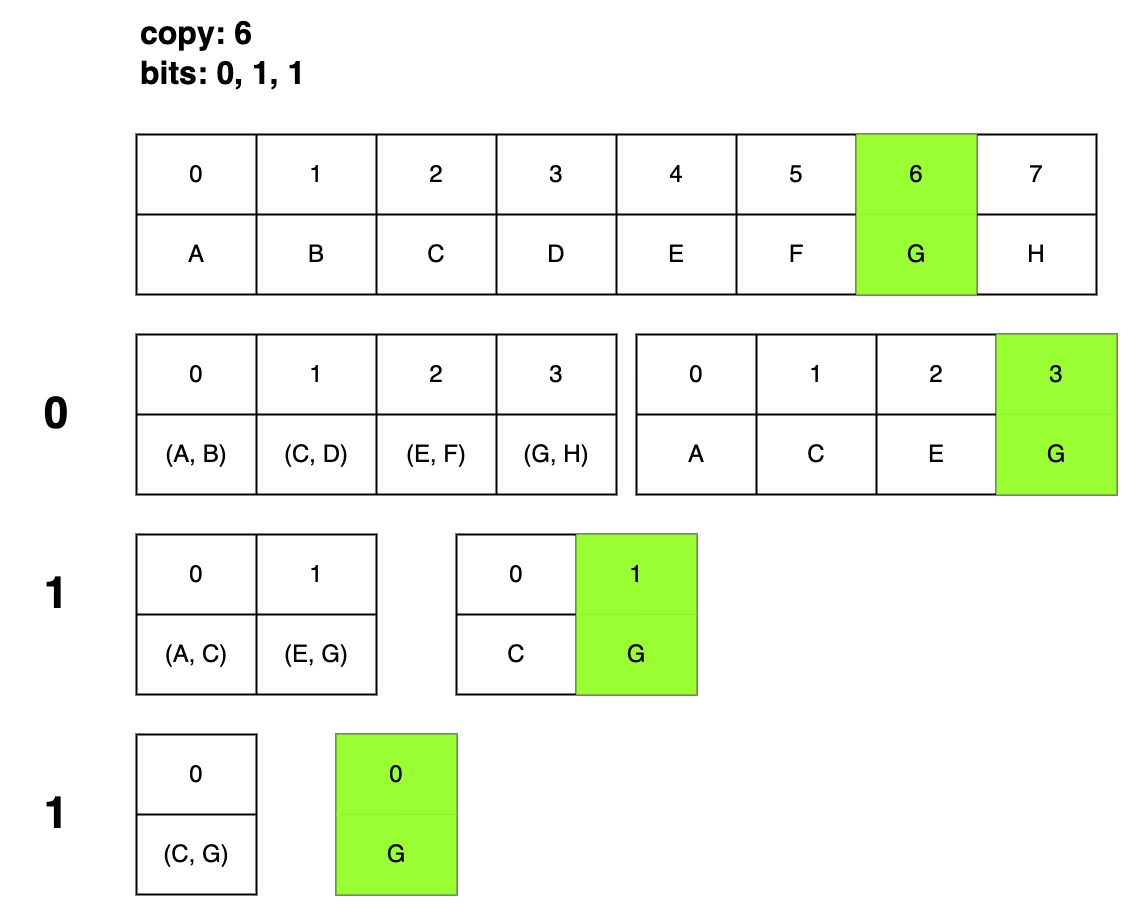
\includegraphics[width=0.6\textwidth]{gates/random_access_example.jpeg}
        \caption{Random Access Example}
        \label{fig:random-access-example}
    \end{figure}
    \begin{lstlisting}[language=rust]
for b in bits {
    list_items = list_items
        .iter()
        .tuples()
        .map(|(&x, &y)| builder.select_ext_generalized(b, y, x))
        .collect()
}
// Check that the one remaining element after the folding is the claimed element.
debug_assert_eq!(list_items.len(), 1);
constraints.push(builder.sub_extension(list_items[0], claimed_element));
    \end{lstlisting}
\end{itemize}

Finally, the constant is constrained -- A total of num\_extra\_constraints constraints.

In summary, there're $\text{num\_copies} \times (\text{bits} + 2) + \text{num\_extra\_constants}$ constraints. Degree is $\text{bits} + 1$ which happens when repeatedly folding the list. 
